\chapter{---------------}
  \textcolor{yellow}{------------------------------------------------}


% =================== %

\subsection{???}

    % 看來 多點 unit 可以切出更細節的資訊 still true, and proved by AP for 50 \\
    % But, this pattern still greatly influenced by basic unit (for APs). \\
    % Histogram 是有在往左跑,但是不是很有意義? \\
    % 跟其他語音的混淆關係反而不那麼明確了……嗎?Plo down but Fri up? \\
    % pur\_cls 提升的很很很少……證明已經沒什麼空間了 \\
    % H(u) 變化不大(除了50ap1k的 S 掉下去了?看看更多?…希望電腦不要死掉)\\
  % each class的pur跟MI改善也很少,除本來差的plosive其他幾乎提升得很有限 \\
    (( 頂多統計 lengths? 但這可以幹嘛?))) → 看 pieces 多時有沒有大塊的?但這要個案探討才有意義吧?

**+ triunits!

%%%%%%%%%%%%%%%%
%%%%%%%%%%%%%%%% [[[[[[[[[[[[[[[[[[[[[[
\textbf{\textcolor{red}{完了,第三章離散單元的個數統計是不是要補上,或者在第四章呈現,if stats!}} <-----
%%%%%%%%%%%%%%%% ]]]]]]]]]]]]]]]]]]]]]]
%%%%%%%%%%%%%%%%

%---------------------------------

    本來想說這很 trivial,但仔細想想 subword 或許會混合本來代表不同 phn 的 units?所以還是維持 pattern 這件事也許……不是那麼 trivial?要在有機會跟人家混淆搞在一起的狀況卻還是維持這個 pattern,挺神奇的 \textcolor{cyan}{→ 來統計「混淆 different phncls 的 piece????」}

{
\begin{figure}
    \centering
    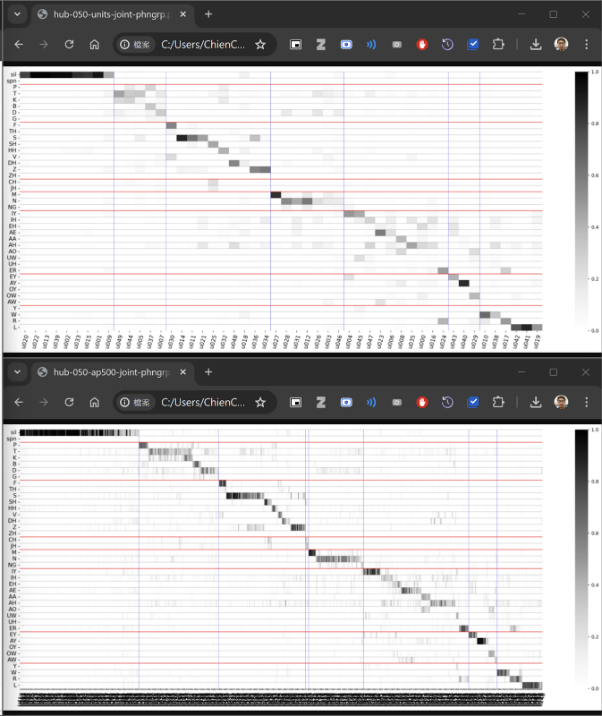
\includegraphics[width=1\linewidth]{feasiblefigs/ch4figs/drafts/1.png}
\end{figure}
}
{
\begin{figure}
    \centering
    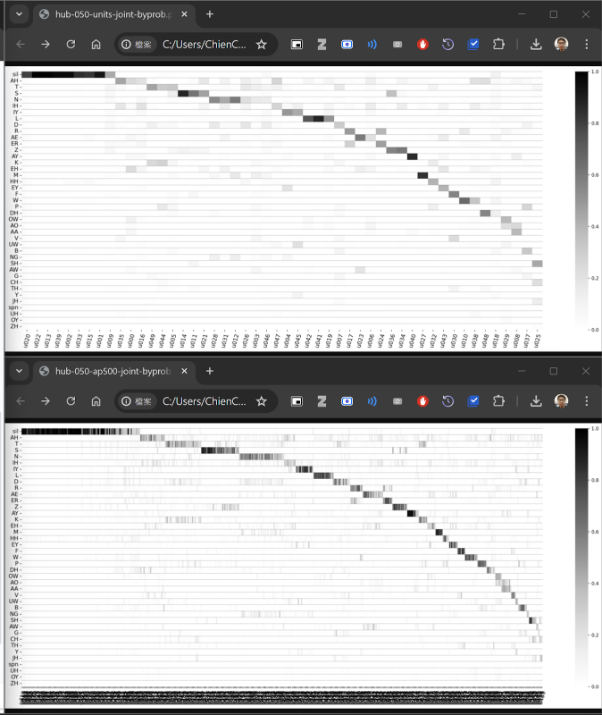
\includegraphics[width=1\linewidth]{feasiblefigs/ch4figs/drafts/2.png}
\end{figure}
}
